\documentclass[PROP_AGutteridge_CS.tex]{subfiles}
\begin{document}

\chapter{Introduction}
\section{Project Background}
Since the actualisation of the World Wide Web, the rate of the spread of ideas, theories and innovations has increased dramatically. Within academia, researchers are able to publish their findings in peer-reviewed academic journals more rapidly than ever before, which are then indexed by databases such as DBLP for the Computer Sciences and PubMed for the Biomedical Sciences. This format, as well as conference proceedings, clinical trial reports and patents, has become progressively more plentiful and accessible due to digitisation. This wealth of information necessitates sophisticated tools to aid users in attaining meaningful results that cannot be derived from the built-in search engine alone: one study has shown that more than a third of PubMed queries return over 100 results\cite{dogan}. The primary aim of this project is to improve the flexibility, and ultimately accuracy, of searching or browsing through scholarly literature. 

\section{Comparison of Bibliographic Resources}
When faced with the task of finding academic literature, researchers may utilise any number of bibliographic databases and search engines available online, that vary in terms of the services provided and the subjects covered. This project focuses on services that at least partially comprise citations concerning the Biomedical Sciences, as I have experience with the current obstacles associated with usage of these.

\noindent \\ It is of primary importance that the usage of data retrieved is covered by the terms and conditions of the service. As the intention is to make the project publicly accessible as a web application, this restriction rules out Web of Science (Thomson Reuters), Scopus and ScienceDirect (both Elsevier). PubMed, Google Scholar and Microsoft Academic Search can all be freely used in a non-commercial setting.

\noindent \subsection{Microsoft Academic Search}
Microsoft Academic Search (MAS, \url{http://academic.research.microsoft.com/}) is a search engine that encompasses citations from multiple fields across academia. Unique IDs of authors and institutions can be retrieved using the API, making MAS an attractive resource for this project. The largest caveat of MAS is that it is a beta release and currently does not appear to be in active development; the latest update dates back to January 2013\cite{microsoft-help} and a blog post from Nature News reported that the number of indexed documents has been in decline since 2010\cite{nature-news}. It is important for the project to be able to access recent publications, and for this reason MAS is not appropriate.

\noindent \subsection{Google Scholar}
Google Scholar (UK, \url{http://scholar.google.co.uk/}) is a search engine that returns ranked journal articles and related materials when queried. It is currently not possible to retrieve the institution address or author keywords, therefore the data is not detailed enough to inform the web application alone. However, one field with potential utility is the number of citations a paper has received. Due to the lack of an API, a scraper such as the open-source Python module scholar.py (\url{https://github.com/ckreibich/scholar.py}) is required to retrieve this data.

\noindent \subsection{PubMed}
PubMed is a database and search engine (\url{http://www.ncbi.nlm.nih.gov/pubmed}) maintained by the National Center for Biotechnology Information (NCBI) as part of the Entrez suite of databases related to health and the Life Sciences. PubMed comprises of citations for a broad range of subjects and resources from the Medical Literature Analysis and Retrieval System Online (MEDLINE) database as well as full-length texts available from PubMed Central. At the time of writing, the home page states that over 24 million citations have been indexed. \\

\noindent Searches carried out on PubMed are directed in part by keywords that have been associated with each publication. These can be listed as Medical Subject Headings (MeSH terms), a medical vocabulary for topics that allows for hierarchical organisation of concepts and disambiguation of terminology\cite{mesh} (Fig.1). This structure provides machine-readable context to an unannotated string, which in this project could allow for more meaningful retrieval and display of results. \\

\noindent Of importance to the implementation of this project, NCBI has built a public API with a RESTful architecture for retrieval of document summaries from PubMed in either XML or JSON format. NCBI has placed an informal limit of 3 requests/second, with large jobs advised to be scheduled outside of 0500-2100 EST\cite{eutils-usage}. This is not restrictive for this project, particularly as a proof-of-concept. A disadvantage of using PubMed is that citations are not tracked, hence the potential for a combined approach with Google Scholar. 

\begin{figure}[ht]
	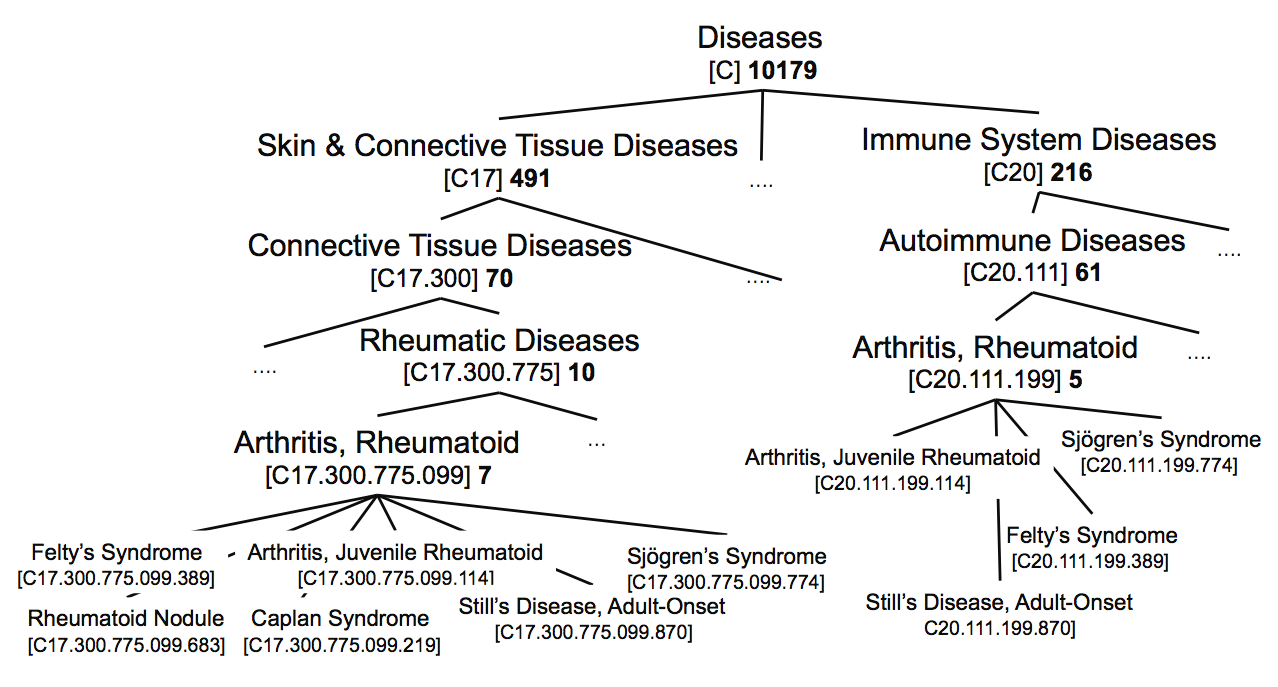
\includegraphics[width=\textwidth]{../lib/images/MeSH}
	\caption{Sample of the hierarchical structure of MeSH terms, centred around rheumatoid arthritis. Each node has a tree number for fast search Taken from \cite{stoyanovich}.}
\end{figure}

\subsection{Discussion}
PubMed is richly detailed, up-to-date both in terms of information and annotation, and accessible to developers with a public API. For these reasons, I have concluded that PubMed is the most pertinent source of data for this project.

\end{document}